%%% Dateikodierung: UTF-8

%%% Magic Comments zum Setzen der korrekten Parameter in kompatiblen IDEs
% !TeX encoding = utf8
% !TeX program = pdflatex 
% !TeX spellcheck = de_DE
% !BIB program = biber

\RequirePackage[utf8]{inputenc} % bei Verw. von lualatex oder xelatex entfernen!
\RequirePackage{hgbpdfa}			% Remove if NO PDF/A output is desired

\documentclass[type=bachelor,theme=default,language=german,titlelanguage=german,smartquotes]{hgbthesis}
% Zulässige Optionen in [..]: 
%    Typ der Arbeit (type=): 'master' (default), 'bachelor', 'diploma', 'phd', 'internship'
%    Theme der Titelseite (theme=): 'default' (default), 'fhooe24'
%    Als Exposé verwenden: 'proposal' oder 'proposal=true' 
%    Hauptsprache im Dokument (language=): 'german' (default), 'english'
%    Sprache der Titelseite (titlelanguage=): 'german', 'english' (default is main language)
%    Umwandlung in typografische Anführungszeichen: 'smartquotes'
%    APA Zitierstil: 'apa'
%    Layout: 'oneside' (einseitig, default), 'twoside' (zweiseitig)
%%%-----------------------------------------------------------------------------

% Overrides
\RequirePackage{./lib/hgb-listings-override}
\RequirePackage{./lib/hgb-bib-override}

% Other Settings
\graphicspath{{images/}}  % Verzeichnis mit Bildern und Grafiken
\bibliography{bib/references} % Biblatex-Literaturdatei (hgbreferences.bib)


%%%-----------------------------------------------------------------------------
\begin{document}
%%%-----------------------------------------------------------------------------

%%%-----------------------------------------------------------------------------
% Angaben für die Titelei (Titelseite, Erklärung etc.)
%%%-----------------------------------------------------------------------------

\title{Aktivitäts-Tracking-Framework}
\subtitle{Design und Implementierung}
\author{Florian Wagner}

\programtype{Fachhochschul-Bachelorstudiengang} % oder Fachhochschul-Bachelorstudiengang
\programname{Software Engineering}
\institution{Fachhochschule Oberösterreich}

\placeofstudy{Hagenberg}
\dateofsubmission{2026}{07}{01} % {JJJJ}{MM}{TT}

% Liste der Betreuungspersonen, bis zu 4 sind möglich, Titel in [] ist optional
\advisor{FH-Prof.~Dipl.-Ing.~(FH)~Dr.~Josef~Pichler}
%\advisor[Zweitbetreuerin]{FH-Prof.\textsuperscript{in} Susanna A.~D. Visor, PhD}

%\license{cc}      % Unter Creative Commons Lizenz veröffentlichen (empfohlen)
\license{strict} % Restriktieve Lizenz, "Alle Rechte vorbehalten"

%%%-----------------------------------------------------------------------------
\frontmatter                                       % Titelei (röm. Seitenzahlen)
%%%-----------------------------------------------------------------------------

\maketitle
\tableofcontents

\chapter{Vorwort}

 % Ein Vorwort ist optional
\chapter{Kurzfassung}
\label{cha:abstract}

\begin{german}

Der schnelle technologische Wandel erfordert von Unternehmen wie der RZL Software GmbH eine kontinuierliche Anpassung und stellt sie vor strategische sowie technische Herausforderungen. Die Umstellung älterer Softwaresysteme bedeutet in der Regel einen enormen Ressourcenaufwand. Hinsichtlich der Effizienz kann eine selektive Auswahl von Funktionalitäten auf Basis pseudonymisierter Nutzerdaten wesentliche Steigerungen bewirken. Des Weiteren können etablierte Prozesse von Anwendern ermittelt, beibehalten und optimiert werden.

Während es im Web bereits bestehende Standardlösungen für dieses Problem gibt, ist dies für komplexe Windows-Forms- und WPF-Rich-Client-Applikationen nicht der Fall. Daher beschäftigt sich diese Arbeit mit der Entwicklung eines Aktivitäts-Tracking-Frameworks, das für WPF- und Windows-Forms-Anwendungen möglichst flexibel eingesetzt werden kann. Dieses Framework soll es ermöglichen, Verhaltensdaten an das Unternehmen zu senden, ohne gravierende Änderungen am bestehenden System vorzunehmen und dabei die Benutzung des Programms nicht zu beeinträchtigen.

Der Einstieg erfolgt mit dem Vergleich verschiedener Technologien. Daraufhin wird das Systemdesign auf Basis dieser Grundlagen erstellt. Anschließend wird das System mittels C\# umgesetzt und zu Testzwecken jeweils in eine WPF- und eine Windows-Forms-Applikation integriert. Um die Funktionsfähigkeit zu demonstrieren, wird eine Konfiguration erstellt und aus dem bestehenden System entsprechende Daten ermittelt. Diese Daten bilden zugleich die Basis für die Beantwortung der Fragen, die sich aufgrund des Optimierungsproblems ergeben haben.

\end{german}

		
\chapter{Abstract}


\begin{english} %switch to English language rules
This should be a 1-page (maximum) "summary" of your work in English.
% ...
\end{english}



%%%-----------------------------------------------------------------------------
\mainmatter                             % Hauptteil (ab hier arab. Seitenzahlen)
%%%-----------------------------------------------------------------------------

\chapter{Einleitung}
\label{cha:introduction}
Dieses Kapitel gibt eine Übersicht über die Motivation und die Ziele dieser Arbeit. 
Des Weiteren wird eine Übersicht über das Vorgehen zur Erreichung des Ziels gegeben.

\section{Hintergrund und Motivation}

\subsection{Umstellung von Softwaresystemen}
Viele Unternehmen stehen vor der Entscheidung, größere Softwaresysteme auf neue Technologien umzustellen. Dies erfordert jedoch häufig einen enormen Entwicklungsaufwand und somit oft mehr Aufwand, als die verfügbaren Ressourcen zulassen, da neben der Umstellung meist noch neue Produkte entwickelt werden. Neben KI, speziellen Tools und anderen technischen Möglichkeiten, Code wiederzuverwenden oder auf eine andere Technologie zu migrieren, ist eine vorerst einfache Möglichkeit Features wegzulassen.

\subsection{Entscheidung für Features}
Die Basis für faktenbasierte Entscheidungen bilden hierbei Verhaltensdaten aus der bestehenden Anwendung. Derartige Daten müssen daher vor solchen Umstellungen mit Tracking-Technologien ermittelt und ausgewertet werden. Im Web gibt es bereits verschiedene Möglichkeiten, gezielt solche Daten zu sammeln und auf einer Weboberfläche darzustellen. Vergleichbare Möglichkeiten existieren im Bereich von Desktopanwendungen, die auf den UI-Frameworks WPF und Windows Forms basieren, nicht. Die Auswertung mit den bestehenden Systemen ist zwar oft unabhängig von der Technologie möglich, jedoch fehlt das Gegenstück zur Sammlung der Daten aus Desktopanwendungen.

\subsection{Technologieänderung Richtung Web}
Aktuelle Trends zeigen, dass sich die Entwicklung Richtung Web verlagert und Desktopanwendungen dadurch an Relevanz verlieren. Daher sind gerade für nicht-webbasierte Technologien Daten über die Nutzung der Software wichtig. Unternehmen wie RZL Software benötigen daher Lösungen, die es ihnen ermöglichen, Nutzungsdaten in WPF- und Windows-Forms-Applikationen zu sammeln und das auf eine möglichst einfache und flexible Art und Weise.

\section{Ziele der Arbeit}

\subsection{Datenermittlung}
Das Ziel der Arbeit ist die Entwicklung eines Verhaltens-Tracking-Frameworks, das für Windows-Forms- und WPF-Anwendungen eingesetzt werden kann. Die Anforderungen an dieses System sind die Ermittlung, Filterung und Extraktion von Nutzungsdaten. Darauf aufbauend müssen die ermittelten Daten pseudonymisiert und strukturiert an ein bestehendes System übermittelt werden können. Daher liegt der Fokus der Arbeit auf der Datenermittlung und nicht der Auswertung oder Darstellung der Daten.

\subsection{Konfigurierbar}
Aus Entwicklungssicht muss eine gezielte Steuerung und Auswahl der zu sendenden Daten einfach und ohne Anpassung des bestehenden Codes möglich sein. Somit entsteht die Voraussetzung einer einmalige Integration in das bestehende System, wobei sich das Framework flexibel durch Konfiguration an das Basissystem anpassen muss.

\subsection{Fragen zur Beantwortung}
\label{subsec:initial_questions}
Von besonderer Relevanz ist, dass die vom System erfassten Informationen die Auszuwertenden dabei unterstützen, folgende Fragen zu beantworten:

\begin{itemize}
    \item Wie oft wird eine Ansicht in der Anwendung geöffnet?
    \item Wie oft wird eine bestimmte Anwendungsmöglichkeit verwendet?
    \item Welche Shortcuts werden in einer Ansicht verwendet?
    \item Wie hoch ist die Anzahl von bestimmten Datensätzen?
    \item Wie beeinflussen Versionsänderungen das Laufzeitverhalten?
    \item Welche Aktionen treten in einer Ansicht auf?
    \item Gibt es eine bestimmte Abfolge von Aktionen im System?
    \item Wie interagieren Nutzer mit einer Ansicht?
\end{itemize}

\subsection{Anwendung des Systems}
Um zu zeigen, dass dieses System die entsprechenden Anforderungen erfüllt, soll diese Arbeit diese Fragen aus Abschnitt \ref{subsec:initial_questions} auf Basis einer Ansicht aus einem bestehenden System beantworten. Somit soll an einem Praxisbeispiel die Verwendung des Frameworks verdeutlicht werden.

\section{Vorgehensweise}
Um ein funktionierendes Framework zu entwickeln, welches die Anforderungen erfüllt, wird nach einem Schema vorgegangen. Dieses Schema ist in diesem Abschnitt beschrieben und hilft dabei, die Anforderungen zu erfüllen.

\subsection{Analyse}
\label{subsec:research}
Im ersten Schritt ist es wesentlich, bestehende Konzepte zu erfassen und auf die verwendete Technologie zu übertragen. Diese Systeme werden größtenteils im Webbereich eingesetzt und sind in Abschnitt \ref{sec:solutions_tracking} zusammengefasst. Aus diesen Grundlagen geht auch hervor, wie wichtig es ist, Cross-Cutting-Concerns \cite{crosscutting} zu berücksichtigen und den bestehenden Code dabei sauber zu halten.

\subsection{Design}
\label{subsec:design_info}
Im nächsten Schritt ist es notwendig, die in Abschnitt \ref{subsec:research} gewonnenen Erkenntnisse in ein möglichst modulares System zu überführen. Dabei wird mit der Konfiguration begonnen, da sie klar beschreibt, welche Aufgaben die anderen Komponenten im System erfüllen müssen. Die Komponenten für die Datenerfassung, das Extrahieren und die Zusammenstellung der Daten folgen anschließend.

\subsection{Implementierung}
Das aus Abschnitt \ref{subsec:design_info} erhaltene Design kann im Anschluss umgesetzt werden. Dabei ergibt sich die zum Testen und Entwickeln sinnvolle Reihenfolge (Konfiguration, Datensammlung und Datenextraktion). Nach dem Verbinden dieser Komponenten zeigt sich, wie diese unabhängigen Teile zusammenspielen. In der Implementierung der Datensammlung erfolgt bereits die Integration in die bestehenden Anwendungen.

\subsection{Konfiguration und Testen}
Um die Funktionsfähigkeit des Systems zu demonstrieren, muss eine praxistaugliche Konfiguration bereitgestellt werden. Die daraus resultierenden Daten werden anschließend verwendet, um die in Abschnitt \ref{subsec:initial_questions} abgeleiteten Fragen zu beantworten.



\chapter{Grundlagen}
\label{cha:grundlagen}

\section{Vergleichbare Anwendungen}
\label{sec:similar_applications}

\subsection{Google Analytics}
\label{subsec:google_analytics}

\subsection{Application Insights}
\label{subsec:applications_insights}

\section{Mögliche Ansätze für Aktivitäts-Tracking}
\label{sec:solutions_tracking}

\subsection{Proxy Server}
\label{subsec:proxy_server}

\subsection{Externes JavaScript}
\label{subsec:external_js}

\subsection{Automatisch generierter Code}
\label{subsec:autogenerated_code}

\subsection{Aufgabendelegation}
\label{subsec:task_delegation}

\section{Softwaremuster für UI Frameworks}
\label{subsec:patterns}

\subsection{MVVM}
\label{subsec:mvvm}

\subsection{MVP}
\label{subsec:mvp}







\chapter{Technologien und Werkzeuge}
\label{cha:technologie_werkzeuge}
Die verwendeten Technologien und Werkzeuge sind für diese Arbeit wesentlich, um die Implementierung nachvollziehen zu können. Die Entwicklungsplattform .NET spielt dabei für das entwickelte Framework eine entscheidende Rolle, wie bereits in Unterabschnitt \ref{subsec:patterns} bei den beschriebenen Patterns erwähnt. In diesem Kapitel werden daher einige zentrale Konzepte vorgestellt.

\section{Visual Studio}
\label{sec:visual_studio}
Für C\# existieren mehrere Entwicklungsumgebungen, wie zum Beispiel Rider \cite{jetbrains-rider} oder Visual Studio \cite{MicrosoftVisualStudioIDE2022}. Da die in dieser Arbeit erstellte Software in einem produktiven Umfeld eingesetzt werden soll, in welchem Visual Studio für die Entwicklung verwendet wird, wird für die Entwicklung ebenfalls Visual Studio 2022 eingesetzt. Visual Studio ist eine komplexe Integrated Development Environment (IDE) von Microsoft und beinhaltet Funktionalitäten zum Erstellen, Debuggen, Testen und weitere nützliche Features.

\section{.NET}
\label{sec:dotnet}
Für die Implementierung in Kapitel \ref{cha:implementierung} wird die von Microsoft bereitgestellte Laufzeitumgebung und Entwicklungsplattform .NET \cite{dotnet} in der Version 8 \footnote{Microsoft veröffentlicht alle zwei Jahre eine Long-Term-Support-Version (LTS) von .NET. Version 8 wurde im November 2024 bereitgestellt und bietet langfristigen Support. Darüber hinaus erscheint jährlich im November eine neue .NET-Version.} verwendet. Diese Version enthält bereits die beiden UI-Frameworks WPF (siehe Unterabschnitt \ref{subsec:WPF}) und Windows Forms (siehe Unterabschnitt \ref{subsec:Winforms}), die ausschließlich unter Windows-Betriebssystemen eingesetzt werden können. Die für diese Arbeit relevanten Konzepte und Funktionen von .NET werden in diesem Kapitel näher erläutert.

\subsection{C\#}
\label{subsec:csharp}
Für die .NET-Plattform stehen mehrere Programmiersprachen zur Verfügung, darunter C\#, F\# und VB.NET. Für die Entwicklung des Frameworks wird C\# verwendet. Microsoft \cite{microsoft-tour-of-csharp} beschreibt C\# als die beliebteste Sprache innerhalb des .NET-Ökosystems, welche auf dem objektorientierten Paradigma aufbaut. Darüber hinaus integriert C\# Konzepte aus weiteren Programmierparadigmen, wie der funktionalen Programmierung. Ein Beispiel für die funktionale Programmierung ist Language Integrated Query (LINQ), das typisierte Abfragen in einer SQL-ähnlichen Syntax direkt im Code ermöglicht.

\subsubsection{Übersetzung und Ausführung}
C\# wird, wie auch andere Sprachen desselben Ökosystems, zunächst in IL (Intermediate Language) übersetzt. Dieser IL-Code wird anschließend durch die Common Language Runtime (CLR) \cite{microsoft-clr-overview} in nativen Maschinencode umgewandelt. Standardmäßig erfolgt diese Übersetzung in .NET über den Just-in-Time-Compiler (JIT). Es existieren jedoch auch Varianten, bei denen Anwendungen bereits teilweise oder vollständig vor der Ausführung in nativen Code kompiliert werden (Ahead-of-Time-Kompilierung \cite{microsoft-native-aot}).

Für die Ausführung von .NET-Programmen wird somit die CLR benötigt, die Bestandteil der .NET Runtime Environment bzw. des .NET SDK ist. Die Assemblies (siehe Unterabschnitt \ref{subsec:assemblies}) werden üblicherweise als \texttt{.dll}- oder \texttt{.exe}-Dateien abgelegt, unterscheiden sich inhaltlich jedoch von C++ Programmen, die nativ kompiliert werden.

\subsection{Nullable Reference Types}
Der bekannte Informatiker Tony Hoare bezeichnete die Einführung von \texttt{null} als seinen größten Fehler, da die dadurch verursachten Probleme enorm seien \cite{hoare_null_video}. Dieses Problem lässt sich bis zu einem gewissen Grad durch die sogenannten Nullable Reference Types \cite{microsoft-nullable-references} lösen. Der Compiler prüft hierbei, ob eine Variable den Wert \texttt{null} annehmen kann und falls dies der Fall ist, muss der Code explizit eine entsprechende Überprüfung vorsehen. Aufgrund der damit verbundenen Reduzierung von NullReferenceException-Fehlern wird dieses Konzept auch in dieser Arbeit verwendet. Entscheidend ist jedoch, dass die durch den Compiler entstehenden Warnings auf Errors umgestellt werden, um die Abdeckung aller entstandenen Nullszenarien zu garantieren.

\subsection{Assemblies}
\label{subsec:assemblies}
Die Erzeugnisse des Kompilierungsprozesses werden in .NET als Assemblies \cite{msdn_assembly_manifest} bezeichnet. Für Assemblies existieren zwei Dateitypen: \texttt{.dll} und \texttt{.exe}. Assemblies des Typs \texttt{.exe} sind ausführbare Dateien, während Assemblies des Typs \texttt{.dll} Klassenbibliotheken bzw. andere Programmteile darstellen, die wiederverwendet werden können.

\subsubsection{Erzeugung von Assemblies}
Abbildung \ref{fig:assemblies_dotnet} zeigt, wie eine Assembly aus mehreren Quelldateien erzeugt wird. Dabei wird das MSBuild-File verwendet, um dem Compiler die erforderlichen Schritte mitzuteilen. Der Compiler erzeugt anschließend aus den Ressourcen und den C\#-Dateien eine Assembly. Dabei werden die Ressourcen, Metadaten und der IL-Code in die resultierende Datei eingebettet.

\begin{figure}[H]
    \centering
    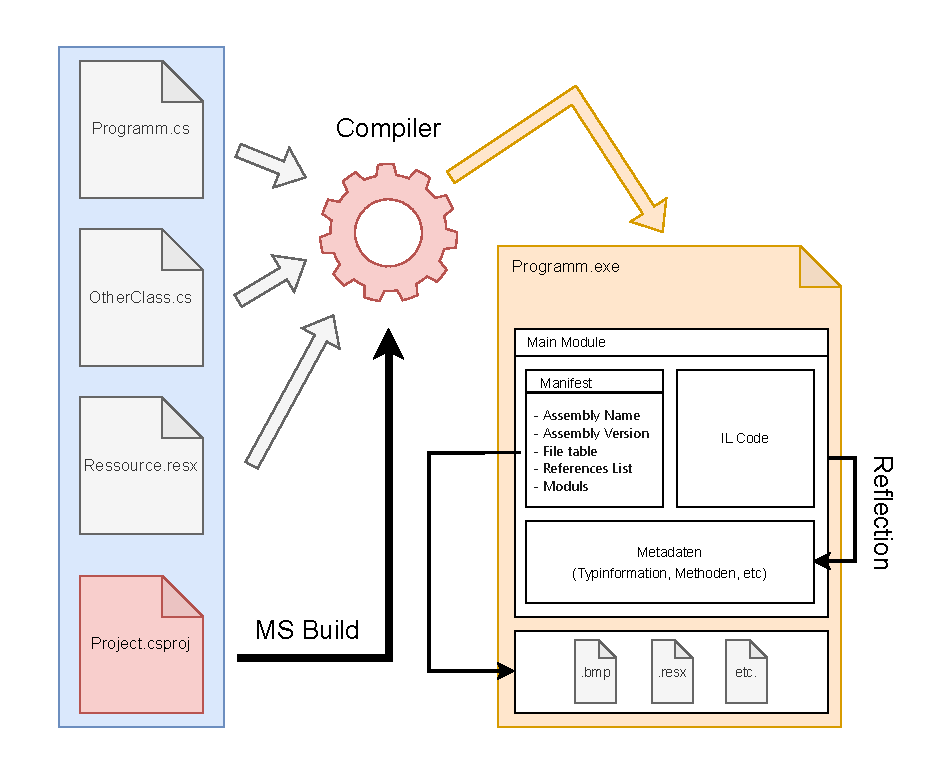
\includegraphics[width=0.9\textwidth]{3_Assemblies_Dotnet}
    \caption{Assemblies Aufbau und Generierung.}
    \label{fig:assemblies_dotnet}
\end{figure}

\subsubsection{Aufbau einer Assembly}
Eine Assembly besteht, wie in Abbildung \ref{fig:assemblies_dotnet} dargestellt, aus mehreren Modulen. Diese sogenannten Module enthalten IL-Code und Metadaten, wobei das Hauptmodul zusätzlich ein Manifest beinhaltet.  
Der IL-Code (Intermediate Language) stellt eine Zwischensprache zwischen Maschinencode und der Programmiersprache dar und enthält die Anweisungen, die letztlich ausgeführt werden.  
Die Metadaten enthalten Informationen über Methodensignaturen, Typen und weitere Strukturdaten. Diese Metainformationen bilden zusammen mit Reflection (siehe Unterabschnitt \ref{subsec:reflection}) einen wichtigen Bestandteil der Laufzeitumgebung. Weiters enthält das erwähnte Manifest folgende Informationen:

\begin{itemize}
    \item Assembly Name
    \item Assembly Version: Wesentlich, da Assemblies die kleinstmögliche Einheit der Versionierung darstellen. Dies ermöglicht beispielsweise die gleichzeitige Verwendung verschiedener Versionen einer Klassenbibliothek in einem Projekt, ohne dass Assemblies überschrieben werden.
    \item File Table: Listet die eingebetteten Ressourcen auf.
    \item References List: Listet die Abhängigkeiten zu anderen Assemblies auf.
    \item Modules: Gibt an, welche Module in einer Assembly enthalten sind. Im Standardfall, wie in Abbildung \ref{fig:assemblies_dotnet} dargestellt, existiert nur ein Modul.
\end{itemize}

Da Assemblies im PE-Format (Portable Executable) \cite{MicrosoftLearn_PEFormat} gespeichert werden, enthalten sie zusätzlich alle für dieses Format erforderlichen Informationen.

\subsection{Reflection}
\label{subsec:reflection}
In Abbildung \ref{fig:assemblies_dotnet} zeigt ein Pfeil vom IL-Code zu den Metadaten. Dies verdeutlicht, dass in C\# ein Mechanismus namens \textit{Reflection} \cite{MicrosoftLearn_Reflection} existiert, der es ermöglicht, Metainformationen über Typen, Methoden oder Attribute zur Laufzeit abzufragen und zu manipulieren. 

Reflection basiert auf speziellen IL-Instruktionen, die über die .NET-API auch in C\# zugänglich sind. Dadurch kann ein Programm beispielsweise alle Eigenschaften eines bestimmten Typs ermitteln und deren Werte dynamisch auslesen oder ändern. 

Reflection ist ein sehr mächtiges Werkzeug, bringt jedoch Leistungseinbußen mit sich. Der Zugriff auf Werte oder Typinformationen über Reflection ist deutlich langsamer als ein zur Compilezeit generierter Zugriff. Das liegt daran, dass die zugrunde liegenden Type- und MemberInfo-Objekte beim ersten Zugriff aus den Assembly-Metadaten erzeugt und anschließend zwischengespeichert werden müssen. Jeder weitere Zugriff erfolgt indirekt über mehrere Objekte, wodurch zusätzliche Zwischenschritte, ähnlich wie bei einer virtuellen Methodentabelle, notwendig werden. Die Auswirkungen von Reflection auf die Laufzeit werden in einem Artikel auf MSDN näher beschrieben \cite{Pobar2005_PerformancePitfalls}.


\subsection{Asynchrone Programmierung}
\label{subsec:async}
Für trackingbasierte Prozesse ist es wichtig, dass diese die Usability des bestehenden Systems nicht beeinträchtigen. Würden Tracking-Abläufe synchron mit der Benutzeroberfläche ausgeführt werden, könnte die UI währenddessen nicht auf Benutzereingaben reagieren. Daher spielt die asynchrone Programmierung eine entscheidende Rolle in dieser Arbeit.

\subsubsection{Grundlegende Funktionsweise}
Um Aufgaben nebenläufig ausführen zu können, bietet .NET die Möglichkeit, Threads zu verwenden. Threads sind leichtgewichtige Prozesse, die denselben Heap teilen, jedoch jeweils über einen eigenen Stack verfügen. Sie sind, abhängig vom Betriebssystem, ein grundlegender Bestandteil des Systems. Threads können zur Laufzeit erzeugt werden und führen dann Methoden wie im Programm \ref{prog:thread_based_programming} gezeigt aus. Nach Abschluss der Methode beendet sich der Thread und die Ressourcen werden vom Betriebssystem freigegeben. Threads sind ein zentraler Bestandteil von .NET und werden in einem Artikel von Microsoft \cite{Microsoft_ThreadsAndThreading} näher beschrieben.

\begin{program}[H]
\begin{CsCode}
Thread workerThread = new Thread(() => Console.WriteLine("Arbeit beendet"));

Console.WriteLine("Starte Arbeit");
workerThread.Start();
\end{CsCode}
\caption{Erzeugen eines Threads}
\label{prog:thread_based_programming}
\end{program}

Da das Erzeugen von Threads Systemressourcen kostet, stellt C\# die ThreadPool-Klasse bereit. Diese erzeugt eine feste Anzahl an Threads, die wiederverwendet werden. Aufgaben werden als Arbeitspakete an diese Threads delegiert. Alle in C\# vorgestellten Konzepte der asynchronen Programmierung nutzen diesen Pool standardmäßig.

\subsubsection{Konzepte der asynchronen Programmierung in C\#}
In C\# existieren mehrere Konzepte, um Abläufe verzahnt (auf einem einzelnen Kern) oder parallel (auf mehreren Kernen) auszuführen, wie im Buch \cite{sarcar2004design} beschrieben. Zu diesen Konzepten zählen:

\begin{itemize}
    \item \textbf{Asynchrones Programmiermodell:} Umsetzung über Delegate.BeginInvoke und Delegate.EndInvoke.
    \item \textbf{Event basiertes asynchrone Muster:} Ein Thread führt eine Aufgabe aus und informiert einen Observer über deren Abschluss.
    \item \textbf{Task basiertes asynchrone Muster:} Ein Task ist eine Einheit, die eine bestimmte Aufgabe ausführt und Informationen über deren Status enthält.
\end{itemize}

In dieser Arbeit wird das Task basierte asynchrone Muster verwendet, da es die Nutzung von async und await ermöglicht.

\subsubsection{Task basierte asynchrone Muster}
Ein Task \cite{Microsoft_TaskClass} repräsentiert eine definierte Aufgabe. Diese wird standardmäßig auf einem Thread aus dem ThreadPool ausgeführt. Ein Task ermöglicht es, auf seine Fertigstellung zu warten oder nach Abschluss eine Fortsetzung auszuführen. Diese Fortsetzung kann im gleichen Synchronization Context oder in einem anderen Kontext erfolgen, um Deadlocks zu vermeiden. Ein Deadlock kann beispielsweise auftreten, wenn auf einen Task blockierend in einem Thread gewartet wird, der jedoch für die Fortsetzung des Tasks erforderlich ist. Ein Beispiel für asynchronen Code wird in Programm \ref{prog:aync_task_based} gezeigt.

\begin{program}[H]
\begin{CsCode}
Console.WriteLine("Arbeit starten");

Task resultTask = Task.Run(async () =>
{
    for (int i = 0; i < 100; i++)
        await Task.Delay(100);

    Console.WriteLine("Arbeit fertiggestellt");
});

Console.WriteLine("Ohne Arbeit fortsetzen");

await resultTask; // alternativ: .Wait() für synchrones Warten
Console.WriteLine("Arbeit sicher fertig");
\end{CsCode}
\caption{Asynchrone Programmierung mit Tasks}
\label{prog:aync_task_based}
\end{program}

\section{UI-Frameworks}
\label{sec:ui_frameworks}
In diesem Abschnitt werden die UI-Frameworks aus der .NET-Umgebung (siehe Abschnitt \ref{sec:dotnet}) vorgestellt, in die das Aktivitäts-Tracking-Framework integriert werden kann. Für diese Frameworks ist insbesondere das Event-System von Bedeutung, da es ein Tracking durch die Verfolgung von Benutzeraktionen, wie z.B. Button-Klicks, ermöglicht.

\subsection{WPF}
\label{subsec:WPF}
Windows Presentation Foundation \cite{microsoft_wpf_overview} ist ein Framework zur Entwicklung von Windows-Desktop-Applikationen. Es baut auf dem in Unterabschnitt \ref{subsec:mvvm} erläuterten MVVM-Muster auf und verwendet für das Erstellen der Ansichten XAML, einen XML-Dialekt. 

Um die UI-Elemente anzusteuern, gibt es eine Code-Behind-Datei, welche eine Partial-Klasse zu der aus dem XAML generierten Klasse darstellt. Dort können Events behandelt oder anderer view-spezifischer Code ausgeführt werden. Dies wird im Buch \cite{james2015pro} näher erläutert und an Beispielen dargestellt.

\subsubsection{Event-System}
Events stellen die Basis für den Zugriff auf das Verhalten in einer Ansicht dar. WPF bietet hierzu Routed Events \cite{microsoft_wpf_routed_events_overview} an. Routed Events sind Events, die im Elementbaum wandern können und die entsprechenden registrierten Handler im Baum informieren. WPF bietet hierfür folgende drei Modelle für das Wandern durch den Baum an:

\begin{itemize}
    \item \textbf{Bubbling}: Das Event wandert von der Source zum Wurzelelement (Window)
    \item \textbf{Tunneling}: Das Event wandert von der Wurzel zur Source
    \item \textbf{Direct}: Nur Handler auf der Source werden über das Ereignis informiert
\end{itemize}

\begin{figure}[H]
    \centering
    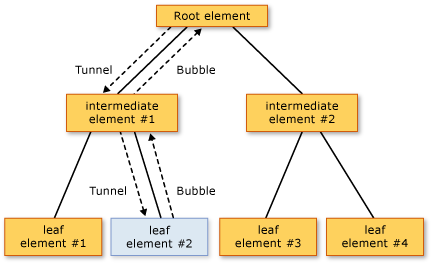
\includegraphics[width=0.6\textwidth]{3_Routed_Events}
    \caption{Reihenfolge Ereignisverarbeitung \cite{microsoft_wpf_routed_events_overview}.}
    \label{fig:routed_events}
\end{figure}

In der Abbildung \ref{fig:routed_events} werden Tunneling und Bubbling durch Pfeile im Elementbaum dargestellt. Dabei soll unter anderem gezeigt werden, dass Preview-Events das Tunneling-Verfahren verwenden und erst anschließend das eigentliche Event über Bubbling propagiert wird.

\subsection{Windows Forms}
\label{subsec:Winforms}
Windows Forms \cite{microsoft_winforms_overview} ist die Vorgängertechnologie von WPF und besteht ebenfalls aus einer Designer-Datei und einer Code-Behind-Datei. Die Designer-Datei enthält dabei direkt Code, der den Aufbau des Steuerelementbaums beschreibt, während die Code-Behind-Datei die Anwendungslogik implementiert. Windows Forms basiert nicht explizit auf einem Design-Muster wie MVVM (siehe Unterabschnitt \ref{subsec:mvvm}). Im zu integrierenden System wird jedoch das MVP-Muster verwendet (siehe Unterabschnitt \ref{subsec:mvp}). Dadurch befindet sich in der Code-Behind-Datei nur noch die für die View notwendige Anzeigelogik.

\subsubsection{Event-System}
Events in Windows Forms \cite{microsoft_winforms_events_overview} sind grundsätzlich nicht routed, sondern werden nur von den am jeweiligen Steuerelement registrierten Event-Handlern verarbeitet. Es gibt jedoch Ausnahmen bei Steuerelementen, die keinen eigenen Fenster-Handle besitzen und daher keine Events direkt empfangen können. In diesen Fällen übernimmt das übergeordnete Steuerelement (Parent) die Ereignisverarbeitung und leitet das Event gegebenenfalls weiter. Solche Events können somit sowohl vom Parent- als auch vom Child-Element behandelt werden. Das Verhalten hängt dabei häufig von Einstellungen wie KeyPreview \cite{microsoft_form_keypreview} ab und muss entsprechend berücksichtigt werden.

Die bereitgestellten Events unterscheiden sich je nach Steuerelement. Abhängig vom Anwendungsfall müssen für die einzelnen Steuerelemente unterschiedliche Handler registriert werden. Die Lifecycle-Events bleiben jedoch weitestgehend gleich.






\chapter{Bestehendes System}
\label{cha:basis}
Da die Arbeit bereits in ein bestehendes System integriert wird, gibt es Möglichkeiten, bereits vorhandenen Code wiederzuverwenden. Um die Implementierung (Kapitel \ref{cha:implementierung}) nachvollziehen zu können, werden in diesem Kapitel einzelne bestehende Konzepte vorgestellt, die dabei helfen, das Framework zu integrieren und weiterzuentwickeln.

\section{MVVM spezifische Erweiterungen}
\label{sec:mvvm_extensions}
Grundsätzlich basiert das WPF-System (siehe Unterabschnitt \ref{subsec:WPF}) auf dem in Unterabschnitt \ref{subsec:mvvm} beschriebenen MVVM-Muster. Würde jedoch die gesamte Logik direkt in die Vererbungshierarchie der ViewModels integriert werden, würde dies die Flexibilität erheblich einschränken und die Komplexität deutlich erhöhen. Daher wurde das MVVM-Muster an die spezifischen Anforderungen der Anwendung angepasst.

\subsection{Presenter}
Bindings ermöglichen zwar einen relativ einfachen Datenaustausch zwischen View und ViewModel, jedoch treten häufig Situationen auf, in denen Daten das Verhalten der View beeinflussen oder Aktionen im ViewModel ausgelöst werden müssen, die sich über einfache Commands\footnote{Commands \cite{wpf_commanding_overview} sind ein Konzept, bei dem ein Objekt erstellt wird, das eine Aufgabe ausführt, wenn es getriggert wird. Dieses Objekt kann über ein Binding ausgetauscht werden.} nicht mehr abbilden lassen. 

In der betreffenden WPF-Anwendung kommen daher Presenter zum Einsatz, die die Kommunikation zwischen ViewModel und View sowohl auf Basis von Daten als auch über Events ermöglichen. Dem Presenter sind sowohl die View als auch das ViewModel bekannt, jedoch können weder View noch ViewModel auf den Presenter zugreifen.

Der Erzeugungsprozess des MVVM-Konstrukts mit Presenter sowie die beschriebenen Zusammenhänge sind in Abbildung \ref{fig:mvvm_with_presenter} dargestellt. Die dort abgebildete ViewModel Region ist ein Control, das die Darstellung eines ViewModels mithilfe der entsprechenden View vornimmt. Die ViewModel Region verwendet eine Factory, um die entsprechenden Presenter zu erzeugen. Die dazugehörigen Informationen, welche View und welcher Presenter für ein bestimmtes ViewModel erzeugt werden sollen, entnimmt die Factory der MVVM-Config. 

Die grünen Pfeile in der Abbildung beschreiben den Datenaustausch über Bindings sowie die Events und Daten, die über den Presenter weitergeleitet werden können, wenn beispielsweise keine Commands oder kein verwendbares Binding zur Verfügung stehen.

\begin{figure}[H]
    \centering
    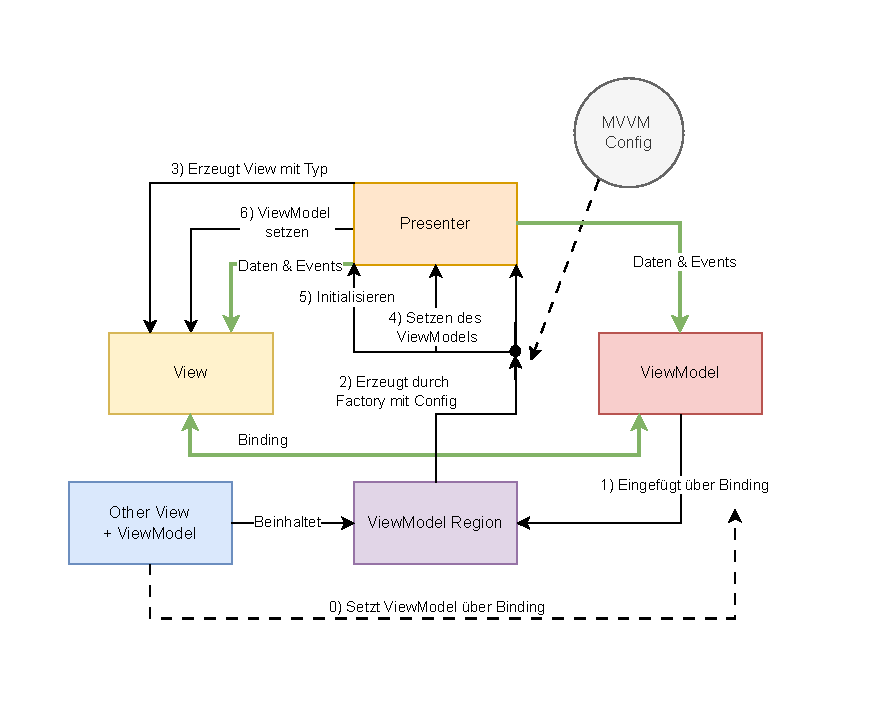
\includegraphics[width=0.8\textwidth]{4_Presenter_MVVM_Extension}
    \caption{Erstellungsprozess und Zusammenhänge des MVVM-Musters mit Presenter.}
    \label{fig:mvvm_with_presenter}
\end{figure}

\subsection{ViewModel Extensions}
\label{subsec:viewmodel_extensions}
ViewModel Extensions erweitern ein ViewModel um zusätzliche Funktionalitäten, wie z.B. automatisches Speichern oder Datenvalidierung. Diese Erweiterungen werden für jedes ViewModel in einer Liste gespeichert und gemeinsam mit dem ViewModel initialisiert. Eine ViewModel Extension erhält Zugriff auf das ViewModel, das sie erweitert und kann über Properties des Haupt-ViewModels auch für das Binding zur View verwendet werden. ViewModel Extensions müssen dem ViewModel während des Konstruktionsprozesses hinzugefügt werden.

\subsection{Presenter und Presenter Extensions}
\label{subsec:presenter_extensions}
Presenter Extensions sind analog zu den zuvor beschriebenen ViewModel Extensions, erweitern jedoch den Presenter. Sie werden über eine Factory in der MVVM-Config\footnote{Die MVVM-Config ist eine Konfiguration, die die Zuordnung von ViewModel, View, Presenter und deren Extensions festlegt.} definiert. Dort können Presenter Extensions mit dem jeweiligen Presenter, der View, dem ViewModel und den zugehörigen ViewModel Extensions erzeugt werden. Presenter Extensions besitzen keine spezielle Struktur und müssen beim Erzeugen initialisiert werden. Wie auch ViewModels werden sie im entsprechenden Presenter gehalten.

\section{Windows Forms spezifische Erweiterungen}
\label{sec:mvp_extensions}
Wie auch in WPF (siehe Unterabschnitt \ref{subsec:WPF}) gibt es für Windows Forms (siehe Unterabschnitt \ref{subsec:Winforms}) einige Erweiterungen, welche die Entwicklung erleichtern und für die Integration des Frameworks in die Anwendung notwendig sind.

\subsection{Embedded Presenter}
\label{subsec:embedded_presenter}
In der mit Windows Forms umgesetzten Anwendung wird das MVP-Muster strikt angewendet. Dennoch gibt es Aufgaben, die sich wiederholen und sich gut aus dem Hauptpresenter herauslösen lassen, um eine höhere Kohäsion zu erreichen. Für solche Aufgaben werden Embedded Presenter eingesetzt. Diese Presenter werden in einem Initialisierungsschritt im Hauptpresenter erzeugt und erhalten Zugriff auf diesen. Dadurch können typische Aufgaben wie Validierung, Speichern oder ähnliches ausgelagert sowie flexibel ausgetauscht oder ergänzt werden. Nach ihrer Erzeugung werden Embedded Presenter unmittelbar initialisiert.

\subsection{UI Accessor}

Um auf Events von Controls zugreifen zu können, wird der UI Accessor verwendet. Dieser abstrahiert verschiedene Events mit gleicher Bedeutung zu einem gemeinsamen, standardisierten Event und ermöglicht dadurch die Registrierung von Handlern auf diese vereinheitlichten Ereignisse. Dies vereinfacht die Handhabung von Benutzerinteraktionen, da bei der Registrierung kein Wissen über das konkrete Event oder den zugehörigen Event-Handler erforderlich ist. Die abstrahierten Events werden über den CommandMapper als sogenannte Commands bereitgestellt und können über den Presenter registriert oder deregistriert werden.

Da es in Windows Forms viele unterschiedliche Events mit gleicher Bedeutung gibt, spielt diese Abstraktion eine wichtige Rolle. Darüber hinaus können auch benutzerdefinierte UserControls mit eigenen Events zentral berücksichtigt werden.

\section{Visual Tree Helper}
\label{sec:visual_tree_helper}
Sowohl in Windows Forms (siehe Unterabschnitt \ref{subsec:Winforms}) als auch in WPF (siehe Unterabschnitt \ref{subsec:WPF}) wird ein Baum aus visuellen Elementen nach dem Prinzip des Composite-Muster aufgebaut (siehe Muster GoF \cite{gamma1995design}).

Gerade für die Registrierung von Events ist das Auffinden bestimmter Controls in diesem Baum entscheidend. Daher gibt es sowohl für WPF als auch für Windows Forms einen Visual Tree Helper, der Elemente rekursiv im Baum findet.

Eine klare Unterscheidung zwischen dem logischen und dem visuellen Baum ist in WPF \cite{microsoft_trees_in_wpf} wesentlich und wird in Abbildung \ref{fig:logical_visual_tree} veranschaulicht. Während der visuelle Baum ausschließlich die tatsächlich sichtbaren Elemente einer Benutzeroberfläche umfasst, beschreibt der logische Baum die hierarchische Struktur der Ansicht, einschließlich jener Objekte, die beispielsweise als Container, Templates oder Datenprovider für sichtbare Elemente dienen.

\begin{figure}[H]
    \centering
    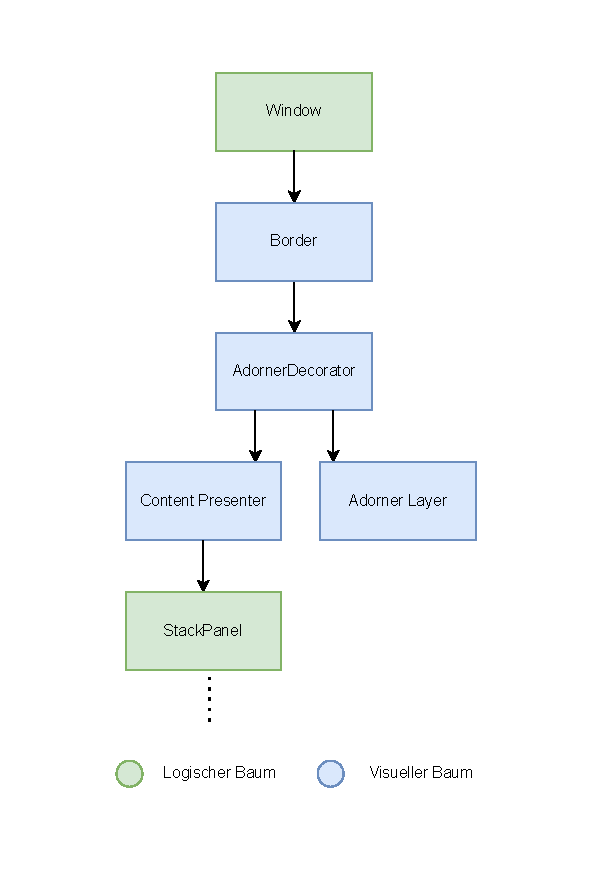
\includegraphics[width=0.5\textwidth]{4_Logical_Visual_Tree}
    \caption{Visueller und logischer Elementbaum.}
    \label{fig:logical_visual_tree}
\end{figure}

\section{AssemblyRegisterResolver}
\label{sec:assembly_resolver}
Für die Konfiguration in Abschnitt \ref{sec:configuration_concept} müssen bestimmte Assemblies (siehe Unterabschnitt \ref{subsec:assemblies}) gefunden werden, die Klassen enthalten, welche ein bestimmtes Interface implementieren.

Da dies insbesondere bei größeren Anwendungen zu Performanceproblemen führen kann, werden alle relevanten Assemblies bereits während des Build-Prozesses auf die Implementierung entsprechender Interfaces überprüft. Die dabei gefundenen Assemblies werden anschließend registriert und in einem Zwischenspeicher abgelegt.

Bei späteren Suchvorgängen nach Klassen, die ein bestimmtes Interface implementieren, müssen dadurch nicht mehr alle Assemblies durchsucht werden, sondern nur diejenigen, die tatsächlich relevant sind. Dies reduziert den Suchaufwand und verbessert die Ladezeit der Anwendung.
\chapter{Konzept}
\label{cha:konzept}
Der Aufbau und das Systemdesign des Aktivitäts-Tracking-Frameworks bilden einen zentralen Bestandteil dieser Arbeit. In diesem Kapitel werden die einzelnen Komponenten beschrieben, die für das Tracking von Aktivitätsdaten erforderlich sind. Die praktische Umsetzung des Konzepts erfolgt anschließend in Kapitel \ref{cha:implementierung}.

\section{Systemarchitektur}
Bevor die einzelnen Komponenten im Detail erläutert werden, beschreibt dieser Abschnitt die Zusammenarbeit und die übergeordnete Struktur der Teilbereiche und Systemkomponenten.

\subsection{Komponenten und Aufbau}

\subsubsection{Teilbereiche und Komponenten}
\label{sec:system_design}
Das Tracking-Framework besteht aus sechs Teilbereichen, die gemeinsam den gesamten Funktionsumfang des Systems abdecken.

\begin{itemize}
    \item Systemkonfiguration
    \item Trackingkonfiguration
    \item Daten- und Aktionsermittlung
    \item Filterung und Extraktion
    \item Vermittlung und Ablaufsteuerung
    \item Datenaustausch und Zwischenspeicherung
\end{itemize}

Im Rahmen der Implementierung (siehe Kapitel \ref{cha:implementierung}) wurden diese Teilbereiche in eigenständige Komponenten unterteilt, sodass alle Aufgaben aus diesen Bereichen berücksichtigt werden. Bestimmte Teilbereiche, wie beispielsweise der Datenaustausch und die Zwischenspeicherung, wurden dabei auf mehrere Komponenten verteilt.

\subsubsection{Struktur der Komponenten}
Abbildung \ref{fig:system_design_components} zeigt, wie die einzelnen Komponenten im System zusammenarbeiten. Das zentrale Element bildet der {Tracking-Manager}, über den alle Komponenten miteinander verbunden sind. Jede Komponente verfügt über eine klar definierte Schnittstelle, die den Zugriff ermöglicht. Nur der Tracking-Manager kennt die einzelnen Komponenten, während diese untereinander vollständig entkoppelt und unabhängig voneinander agieren. Die einzige Komponente, die von mehreren Komponenten genutzt wird, ist die Systemkonfiguration. Sie wird vom Tracking-Manager verwaltet und an die jeweiligen Komponenten weitergegeben.

Diese Struktur sorgt für eine hohe Flexibilität. Änderungen, die von der Systemumgebung abhängen, können vorgenommen werden, ohne andere Teile des Frameworks zu beeinflussen. So lässt sich beispielsweise die Art der Datenverarbeitung anpassen, ohne dass der übrige Aufbau geändert werden muss.

\begin{figure}[H]
    \centering
    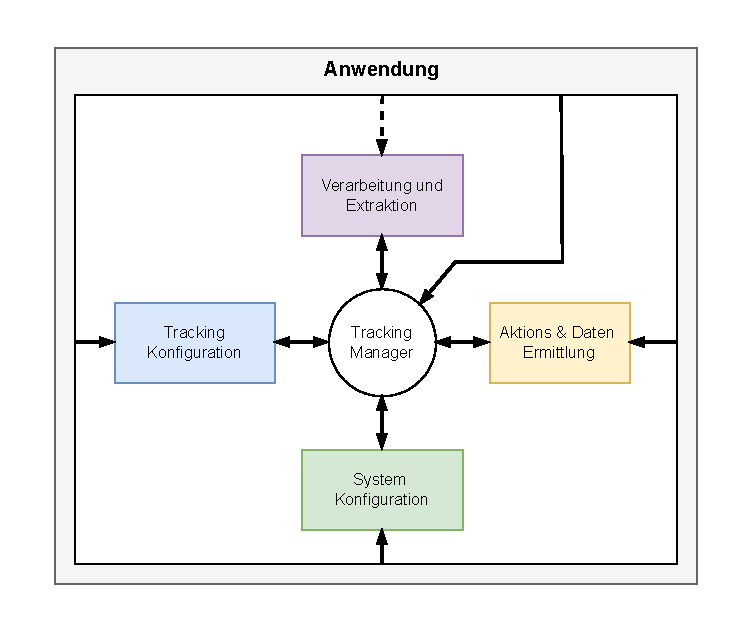
\includegraphics[width=0.65\textwidth]{5_Systemdesign_Components_Tracking}
    \caption{Zusammenhänge der Komponenten im Tracking-Framework.}
    \label{fig:system_design_components}
\end{figure}

Die lose Kopplung besteht nicht nur zwischen den internen Komponenten des Frameworks, sondern auch zwischen der Anwendung und dem Framework selbst. Die Anwendung stellt die Tracking-Konfiguration, Anwendungsdaten sowie eine Systemkonfiguration bereit. Optional kann sie auch Funktionen zum Filtern und Extrahieren übernehmen.
Diese Daten werden über eine definierte Schnittstelle sowie vordefinierte Komponenten und Templates an das Framework übermittelt. Dadurch wird sichergestellt, dass für die Integration nur minimale Kenntnisse über das Framework erforderlich sind. In den meisten Fällen erkennt das Framework seine Abhängigkeiten zur Anwendung selbstständig.

Die Anwendung selbst muss im Wesentlichen lediglich die erforderlichen Daten über eine definierte Schnittstelle bereitstellen. Dadurch lässt sich das System flexibel in unterschiedlichen Technologien einsetzen, beispielsweise in WPF (siehe Unterabschnitt \ref{subsec:WPF}) oder Windows Forms (siehe Unterabschnitt \ref{subsec:Winforms}).

\subsection{Kommunikation zwischen Komponenten}
\label{subsec:communication_between_coponents}

\subsubsection{Kommunikationsgrundlage}
Damit ein Informationsaustausch zwischen den Komponenten möglich ist, wird eine gemeinsame Kommunikationsbasis benötigt. Diese Grundlage besteht aus Objekten, die die gemeinsame Sprache für den Datenaustausch definieren.  
Konzeptionell wird zwischen fünf Informationskategorien unterschieden:

\begin{itemize}
    \item \textbf{Trackingaktionen}: Repräsentieren auftretende Ereignisse innerhalb der Anwendung.
    \item \textbf{Trackingdaten}: Umfassen Daten, die auf Basis einer aufgetretenen Aktion erfasst werden.
    \item \textbf{Extraktionsaufgaben}: Beschreiben, welche Informationen aus Trackingaktionen und Trackingdaten ermittelt werden sollen, und stellen Metadaten für die resultierenden Extraktionsdaten bereit.
    \item \textbf{Trackingaufgaben}: Legen fest, welche Daten für die Weiterverarbeitung ermittelt und verarbeitet werden dürfen.
    \item \textbf{Extraktionsdaten}: Enthalten die aus Trackingaktionen und Trackingdaten extrahierten Informationen, die anschließend weiterverarbeitet oder übermittelt werden können.
\end{itemize}

Die einzelnen Kategorien können verschiedene Objekttypen enthalten, die je nach Anwendungsfall unterschiedlich ausgestaltet sind. Diese Objekte bilden einen grundsätzlich unveränderlichen Standard, wobei Extraktionsdaten, Trackingaktionen und Trackingdaten durch benutzerdefinierte Objekte erweitert werden können. Damit die Daten vom Framework verarbeitet werden können, müssen sie, ähnlich wie bei Google Analytics (siehe Unterabschnitt \ref{subsec:google_analytics}), einer festgelegten Struktur entsprechen.

\subsubsection{Datenübertragungswege}
Der Datenaustausch zwischen den Komponenten kann entweder direkt über Rückgabewerte von Funktionen oder über sogenannte Datenkanäle erfolgen.  
Ein Datenkanal ist im Rahmen dieser Arbeit als ein Konstrukt zu verstehen, über das Daten an eine unbekannte oder externe Komponente weitergegeben werden können.  
Durch die Systemkonfiguration (siehe Abschnitt \ref{sec:integration_concept}) kann die Anwendung verschiedene Wege der Veröffentlichung oder des Bezugs von Daten anbieten. Auf diese Weise bleibt das System flexibel gegenüber unterschiedlichen Datenquellen und Zielen.

\subsubsection{Ablauf der Kommunikation}
Der Ablauf der Kommunikation erfolgt über die zuvor beschriebenen Datenobjekte und wird im in Abbildung \ref{fig:sequence_diagram_communication_components} dargestellten Sequenzdiagramm veranschaulicht.  
Wie dort gezeigt, erzeugt die Anwendung zunächst alle benötigten Komponenten. Die Reihenfolge ergibt sich aus den jeweiligen Abhängigkeiten, wobei die genaue Erstellungsreihenfolge zwischen Datenermittlung (Abschnitt \ref{sec:data_collection_concept}), Verarbeitung (Abschnitt \ref{sec:data_extraction_concept}) und Trackingkonfiguration (Abschnitt \ref{sec:configuration_concept}) nicht entscheidend ist.  

Nach der Erzeugung wird der Tracking-Manager initialisiert. Während dieser Initialisierung wird auch die Systemkonfiguration (siehe Abschnitt \ref{sec:integration_concept}) übergeben. Anschließend initialisiert der Tracking-Manager die Trackingkonfiguration, die wiederum die benötigten Assemblies für die Konfiguration ermittelt. Danach kann der Tracking-Manager die Aufgaben für das Tracking anfordern. Diese Aufgaben werden bei der Initialisierung der Komponenten für Datenermittlung sowie für Verarbeitung und Extraktion berücksichtigt.

\begin{figure}[H]
    \centering
    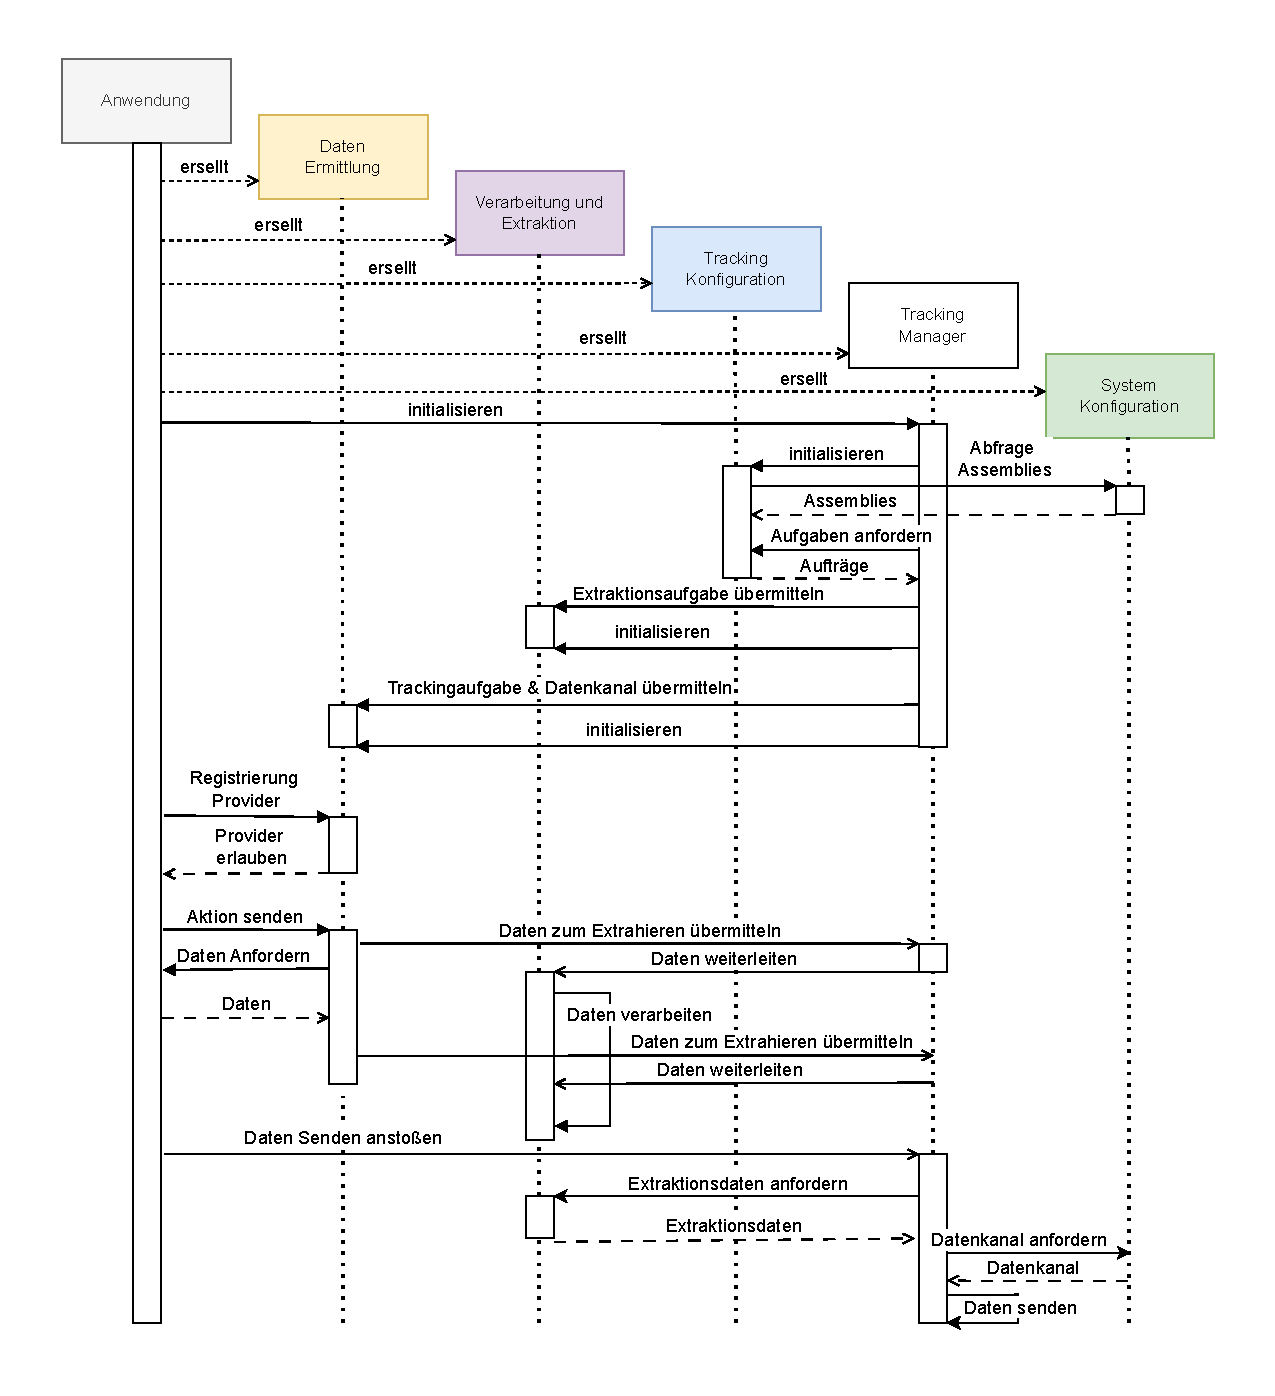
\includegraphics[width=1.0\textwidth]{5_Sequence_Diagram_Components_Communication}
    \caption{Ablauf der Kommunikation zwischen den Komponenten.}
    \label{fig:sequence_diagram_communication_components}
\end{figure}

Nach Abschluss der Initialisierung kann die Anwendung sogenannte Data Provider registrieren. Dabei entscheidet die Komponente zur Datenermittlung, ob ein Provider einen entsprechenden Datenkanal zur Übertragung von Daten erhält. Über diesen Kanal können sowohl Aktivitätsdaten als auch nachgelieferte Daten gesendet werden.

Die übergebenen Daten werden anschließend in der Extraktionskomponente asynchron zur Anwendung empfangen und weiterverarbeitet.  

Wenn die Anwendung das Ausliefern der Daten anstößt, fordert der Tracking-Manager die Extraktionsdaten an und übergibt sie über den in der Systemkonfiguration bereitgestellten Datenkanal an die entsprechende Zielkomponente.

\section{Tracking-Konfiguration}
\label{sec:configuration_concept}
Wie bei Google Analytics (siehe Unterabschnitt \ref{subsec:google_analytics}) und OpenTelemetry (siehe Unterabschnitt \ref{subsec:open_telemetry}) verfügt auch dieses Framework über eine Konfiguration, in der festgelegt wird, welche Daten getrackt werden sollen. Für das hier vorgestellte Framework ist eine hybride Lösung vorgesehen, die sowohl Online-Konfigurationen, wie bei Google Analytics, als auch Code-basierte Konfigurationen, wie bei OpenTelemetry, ermöglicht. In dieser Arbeit wird jedoch ausschließlich die zweite Variante konzipiert und umgesetzt.

\subsection{Aufbau der Konfigurationskomponente}
Der Aufbau der Konfigurationskomponente ist in Abbildung \ref{fig:configuration_component} dargestellt. Diese Komponente besteht aus einem Manager, der sowohl für die Initialisierung als auch für die Bereitstellung der Aufgaben verantwortlich ist. Der Manager agiert dabei als Slave des Hauptmanagers.

Das Erstellen der Konfiguration erfolgt durch sogenannte Configuration Builder, die zuvor über eine Fluent API \footnote{Unter einer Fluent API oder auch einem Fluent Interface \cite{Fowler2005FluentInterface} versteht man eine Methodik des Method-Chaining, bei der Konfigurationen in einer flüssigen, satzähnlichen Syntax formuliert werden können.} definiert werden. Optional soll die Komponente so erweitert werden können, dass künftig auch ein Konfigurationsserver angebunden werden kann. Im Rahmen dieser Arbeit bleibt dies jedoch unberücksichtigt.

\begin{figure}[H]
    \centering
    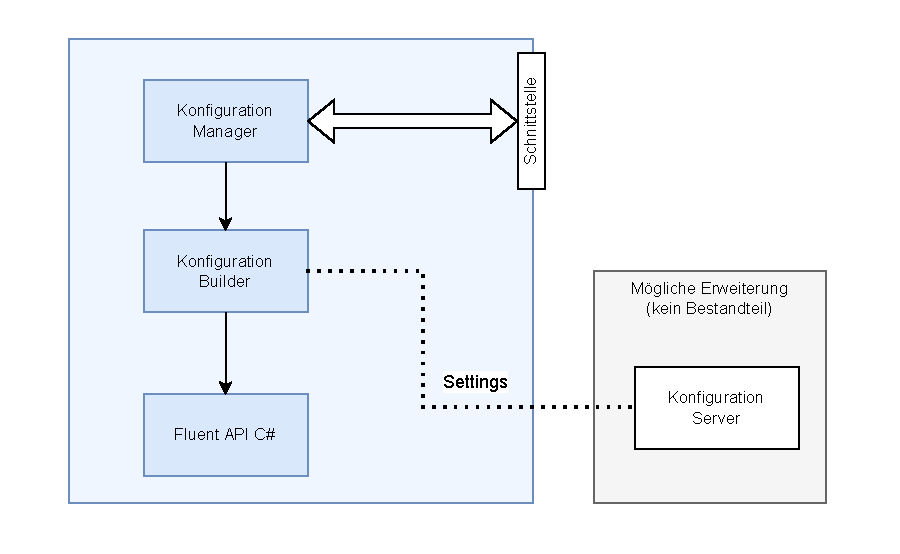
\includegraphics[width=0.55\textwidth]{5_Configuration_Component}
    \caption{Aufbau der Konfigurationskomponente}
    \label{fig:configuration_component}
\end{figure}

\subsection{Konfigurationsmöglichkeiten und Fluent API}

\subsubsection{Kategorien von Informationen}
Um die ursprünglich definierten Fragen (siehe Unterabschnitt \ref{subsec:initial_questions}) beantworten zu können, müssen bestimmte Informationen gesammelt werden. Diese lassen sich in folgende Kategorien einteilen:

\begin{itemize}
    \item \textbf{Metriken:} Zahlenbasierte Daten, wie sie bereits im Zusammenhang mit OpenTelemetry beschrieben wurden. Beispiele hierfür sind die Ladezeit einer Ansicht oder die Anzahl der Öffnungen einer bestimmten Ansicht.
    \item \textbf{Daten:} Informationen, die beispielsweise aus einer Ansicht extrahiert werden können, etwa die Anzahl der Einträge in einer Liste.
    \item \textbf{Nutzung:} Informationen, die Aufschluss über das Nutzungsverhalten der Anwendung geben, beispielsweise wie häufig ein Shortcut in einer bestimmten Ansicht verwendet wird.
    \item \textbf{Workflows:} Informationen, die mit Traces in OpenTelemetry vergleichbar sind und einen Ablauf von aufeinanderfolgenden Aktionen darstellen.
\end{itemize}

\subsubsection{Aufbau der Fluent API}
Die zuvor kategorisierten Daten können weiter beschrieben werden, woraus sich ein Schema ableiten lässt, das für den Aufbau der Fluent API von zentraler Bedeutung ist.\\
\\
$Kontext \rightarrow Kategorie \rightarrow Kategorieoptionen$\\
\\
Daten stammen stets aus einem bestimmten Kontext und gehören zu einer der oben definierten Kategorien. Diese Daten können anschließend durch spezifische Optionen weiter unterteilt werden. Ein vereinfachter Ausschnitt der Fluent API nach diesem Schema wird in Abbildung~\ref{fig:configuration_component_fluent_api} als Syntaxdiagramm dargestellt. Mit der in der Abbildung gezeigten API ist es möglich, das Anfordern von Daten aus einer Ansicht zu konfigurieren.

\begin{figure}[H]
    \centering
    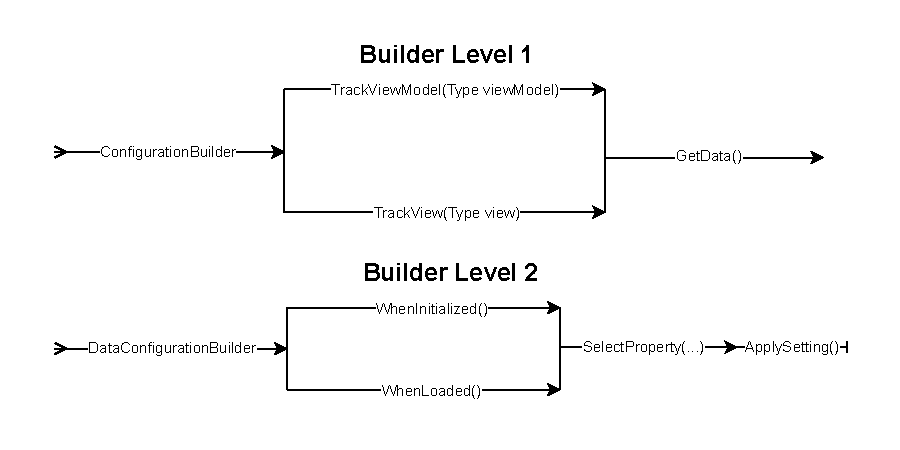
\includegraphics[width=0.82\textwidth]{5_Configuration_Component_Fluent_API}
    \caption{Vereinfachter Ausschnitt der Fluent API für die Tracking-Konfiguration.}
    \label{fig:configuration_component_fluent_api}
\end{figure}

\subsection{Builder und deren Funktionsweise}
Builder \cite{sarcar2004design} sind spezielle Klassen, die konfiguriert werden können und anschließend durch den Aufruf einer Build-Methode entsprechende Objekte erzeugen. Nach der Erzeugung können diese Objekte vom Builder abgerufen werden. Der Director ist die Komponente, die den Erstellungsprozess steuert. Im Kontext dieser Arbeit übernimmt der Manager diese Rolle.

\subsubsection{Bessere Aufgabenteilung durch mehrstufige Builder}
In Abbildung \ref{fig:configuration_component_fluent_api} ist von zwei Builder-Leveln die Rede. Der Grund dafür liegt darin, dass ein einzelner Builder sehr umfangreich und unübersichtlich werden würde. Um die Wartbarkeit und Erweiterbarkeit zu verbessern, werden die Builder daher in mehrere Ebenen unterteilt.  
Der Builder der ersten Ebene ruft die Build Methode der nachfolgenden Ebenen auf und fügt deren Ergebnisse zusammen. Dieses Prinzip folgt dem Composite-Muster \cite{gamma1995design}.

\subsection{Settings und deren Zusammenhang mit Builder}
Aus Sicht der Anwender*innen der API existieren keine Builder direkt. Die Fluent API verwendet stattdessen bestimmte Settings, die am Ende einem Builder hinzugefügt werden. Auf Grundlage dieser Einstellungen kann der Builder anschließend die entsprechenden Objekte erstellen, beispielsweise die Aufgaben zur Datenermittlung (siehe Abschnitt~\ref{sec:data_collection_concept}) und zur Extraktion der Daten (siehe Abschnitt~\ref{sec:data_extraction_concept}).  
Dieser Zusammenhang wird in Abbildung \ref{fig:builder_and_settings_cooperation} dargestellt.

\begin{figure}[H]
    \centering
    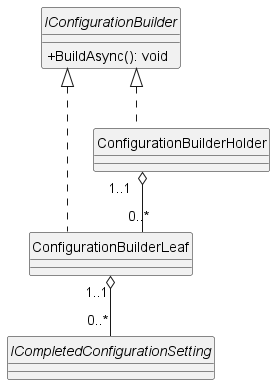
\includegraphics[width=0.4\textwidth]{5_Configuration_Concept_Builder_Class_Diagramm}
    \caption{Klassendiagramm für den Zusammenhang zwischen Builder und Settings.}
    \label{fig:builder_and_settings_cooperation}
\end{figure}

\subsection{Bereitstellen von Einstellungen}
Wie bereits erläutert, werden Einstellungen über eine Fluent-API konfiguriert und einem Builder hinzugefügt. Da Softwaresysteme häufig sehr umfangreich sind, werden sie meist in kleinere Teilprojekte unterteilt. Die in dieser Arbeit behandelte Integration (siehe Kapitel \ref{cha:implementierung}) bezieht sich genau auf ein solches System.

Aus diesem Grund erfolgt die Konfiguration auf Assembly-Basis (siehe Abschnitt \ref{subsec:assemblies}). Konkret bedeutet das, dass pro Assembly mehrere Settings-Provider existieren können, die beim Erstellen einer Konfiguration ausgelesen werden. Diese Provider erhalten eine Starteinstellung (den Einstiegspunkt der Fluent-API) und wenden die entsprechenden Einstellungen automatisch über die API auf einen Builder an.

Diese Provider werden von den Entwickler*innen implementiert, indem die Fluent-API wiederholt auf die jeweilige Starteinstellung angewendet wird. Dabei wird festgelegt, welche Informationen aus dem jeweiligen Teil der Anwendung (der sich in derselben Assembly befinden muss) ermittelt werden sollen.

\section{Daten- und Aktionsermittlung}
\label{sec:data_collection_concept}
Auf Basis der Konfiguration wird, wie bereits beschrieben, ein Tracking-Auftrag erteilt. Dieser Auftrag kann anschließend von der Anwendung abgearbeitet werden. Wie diese Abarbeitung im Detail erfolgt, wird in diesem Abschnitt erläutert.

\subsection{Komponentenstruktur und Aufgabenverteilung}
\label{subsec:data_collection_components}
Abbildung \ref{fig:structure_data_collection} zeigt die Struktur der Daten- und Aktionsermittlungskomponente. Teile dieser Struktur wie die Provider befinden sich innerhalb der Anwendung, während ein Manager die Integration in das Trackingsystem übernimmt. In diesem Unterabschnitt wird dargestellt, welchen Beitrag die einzelnen Bestandteile zur Datenermittlung leisten.

\begin{figure}[H]
\centering
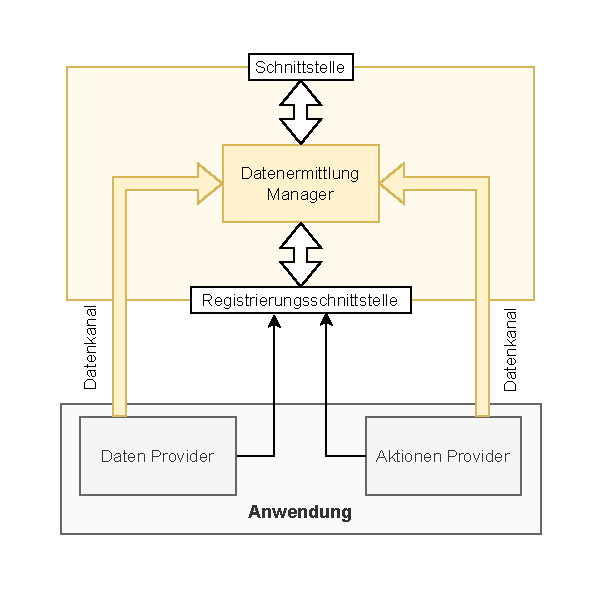
\includegraphics[width=0.52\textwidth]{5_Data_Collection_Structure.pdf}
\caption{Struktur der Datenermittlungskomponente.}
\label{fig:structure_data_collection}
\end{figure}

\subsubsection{Manager für Datenermittlung}
Zunächst ist entscheidend, dass in diesem Kontext unter Datenermittlung sowohl die Erfassung von Aktionen als auch der daraus resultierenden Daten verstanden wird. Der Manager übernimmt daher die Aufgabe, die Zugangskontrolle für beide Arten von Providern sicherzustellen. Dabei wird geprüft, ob ein Provider einen Beitrag zum jeweiligen Tracking-Auftrag leisten kann. Ist dies der Fall, bestätigt der Manager die Teilnahme des Providers durch die Bereitstellung eines Datenkanals.

Wenn anschließend Aktionen über diesen Datenkanal übermittelt werden, ist es die Aufgabe des Managers, die entsprechenden DataProvider zu informieren und die Ermittlung der zugehörigen Daten auszulösen.

Der Datenkanal wird vom Manager wiederum an einen übergeordneten Datenkanal weitergeleitet, der vom Hauptmanager bereitgestellt wird. Damit ist der Manager dem Hauptmanager untergeordnet, analog zum Aufbau beim Konfigurationsmanager.

Insgesamt verwaltet der Manager somit die Tracking-Aufträge und stellt sicher, dass diese ordnungsgemäß und vollständig ausgeführt werden, wie in Abbildung \ref{fig:structure_data_collection} dargestellt ist.

\subsubsection{Provider für Aktionen}
Aktionen sind, wie bereits in Unterabschnitt \ref{subsec:communication_between_coponents} beschrieben, ein wesentlicher Bestandteil der Kommunikation von Ereignissen innerhalb der Anwendung. Sie werden von speziellen Action Providern bereitgestellt, sofern dies vom Manager für Datenermittlung vorgesehen ist.

Die Aktionen werden im jeweiligen Provider über eine Fabrikkomponente erzeugt, deren Implementierung je nach System variieren kann. Provider sind nur aktiv, wenn ihre Registrierung beim zugehörigen Manager erfolgreich abgeschlossen wurde.

Die Übergabe der Aktionen erfolgt nach dem Push-Prinzip, um eine asynchrone Weiterverarbeitung und Filterung zu ermöglichen. Dadurch soll verhindert werden, dass es zu spürbaren Verzögerungen in der Benutzeroberfläche der Anwendung kommt.

Es existiert eine vorgegebene Menge an Providern, die für das korrekte Funktionieren des Frameworks erforderlich sind. Darüber hinaus können jedoch beliebige weitere Provider integriert werden. Auf die vordefinierten Provider wird in Unterabschnitt \ref{subsec:required_provider_and_data} näher eingegangen.

\subsubsection{Provider für nachfolgende Daten}
Wie bereits erwähnt, können Daten auf Basis von Aktionen ermittelt werden. Diese Daten werden über Standard-Datenprovider bereitgestellt. Dabei müssen diese Provider nicht zwingend auf Aktionen reagieren, sie können auch unabhängig davon Daten ermitteln.

Der Standardfall besteht jedoch darin, dass Daten infolge von Aktionen über den zugehörigen Manager angefordert werden (z.B. Property-Daten, nachdem eine Komponente der Anwendung initialisiert wurde). Eine Registrierung, wie sie auch bei den Action Providern erforderlich ist, ist ebenfalls notwendig. Provider sind somit nur aktiv, wenn sie laut Konfiguration (siehe Abschnitt \ref{sec:configuration_concept}) tatsächlich benötigt werden.

Der Aufbau der Datenprovider für nachfolgende Daten ist dem der Action Provider sehr ähnlich und wird daher ebenfalls in Unterabschnitt \ref{subsec:required_provider_and_data} beschrieben. Auch hier existiert eine festgelegte Menge an Providern, die für das ordnungsgemäße Funktionieren der Anwendung erforderlich sind.

\subsection{Benötigte Daten und Provider}
\label{subsec:required_provider_and_data}
Das Framework arbeitet nach dem Prinzip, dass ausschließlich die Daten verarbeitet werden, die auch bereitgestellt werden. Fehlt daher die Implementierung bestimmter Provider, kann die Qualität der Ergebnisse schwanken, da konfigurierte Aufträge unter Umständen nicht vollständig erfüllt werden.

Soll der volle Funktionsumfang des Frameworks genutzt werden, müssen bestimmte vordefinierte Provider implementiert werden. Dabei kann entweder das bereitgestellte Schema verwendet oder eine eigene Implementierung nach demselben Muster erstellt werden.

\subsubsection{Benötigte Provider für Aktionen}
Für die nachfolgend aufgelisteten Aktionen müssen Provider implementiert werden, um den vollständigen Funktionsumfang des Frameworks sicherzustellen:

\begin{itemize}
    \item Aktionen zum Zustand von View und PresentationModel (z. B. initialisiert, geladen)
    \item Aktionen mit Informationen zu den in einer Ansicht verwendeten Shortcuts
    \item Aktionen, die Ereignisse beschreiben, die auf Steuerelementen ausgeführt werden
    \item Aktionen, die die Nutzung bestimmter Funktionen bestätigen (z. B. das Öffnen einer Ansicht zur Datenverarbeitung)
\end{itemize}

\subsubsection{Benötigte Provider für sonstige Daten}
Im vollen Funktionsumfang sollen außerdem die folgenden Datentypen ermittelt werden. Auch hierfür sind entsprechende Datenprovider erforderlich:

\begin{itemize}
    \item Daten zur Ladezeit einer Ansicht
    \item Daten aus der Ansicht selbst, beispielsweise Informationen zu Properties
\end{itemize}

\subsubsection{Schema für Provider}
Die grundlegende Ermittlung der Daten folgt im Wesentlichen stets demselben Ablauf. Aus diesem Grund wird für die benötigten Daten ein Provider-Template bereitgestellt.

Diese Templates orientieren sich am Grundgedanken des Template-Methoden-Musters (siehe Design Patterns der Gang of Four \cite{gamma1995design}). Dabei müssen bestimmte Methoden von den Implementierenden konkret ausgearbeitet werden, um die gewünschten Aktionen in den übergeordneten Algorithmus einzubinden.

Der zugrunde liegende Algorithmus übernimmt anschließend die eigentliche Datenermittlung und stellt die gewonnenen Informationen über den entsprechenden Datenkanal bereit.

Abbildung \ref{fig:structure_data_provider} veranschaulicht die möglichen Strukturen und Implementierungsvarianten für Datenprovider innerhalb dieses Schemas.

\begin{figure}[H]
\centering
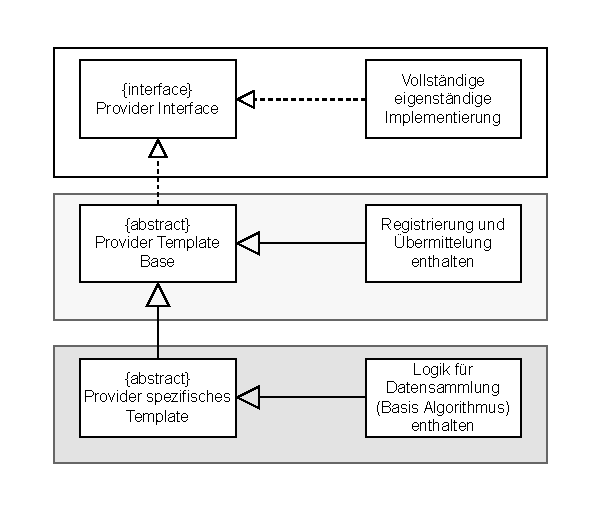
\includegraphics[width=0.52\textwidth]{5_Data_Provider_Structure.pdf}
\caption{Schema für Datenprovider.}
\label{fig:structure_data_provider}
\end{figure}

Wie in Abbildung \ref{fig:structure_data_provider} dargestellt, besteht die Möglichkeit, eigene Implementierungen von Providern zu erstellen. Dennoch wird empfohlen, mindestens den zweiten Layer des Frameworks zu verwenden. Die Basisimplementierung übernimmt bereits die Fehlerbehandlung und das Exception Handling, wodurch mögliche Fehlersituationen automatisch abgefangen werden.

Für den ersten Layer hingegen sind detaillierte Kenntnisse über den Tracking Manager erforderlich, da in dieser Ebene die Registrierung der Provider manuell erfolgen muss.

Für die Standard-Provider sollten daher unbedingt die bereitgestellten Templates verwendet werden, da diese ausreichende Flexibilität bieten und gleichzeitig eine robuste sowie einheitliche Implementierung sicherstellen.

\section{Filterung und Extraktion}
\label{sec:data_extraction_concept}
Wie bereits im Unterabschnitt \ref{subsec:data_collection_components} beschrieben, werden die Daten während der Sammlung nach dem Push-Prinzip weitergegeben, ohne dass zuvor eine Filterung oder Aggregation erfolgt. Dieses Vorgehen hat Performance-Vorteile, da die Übertragungszeit in der Regel kürzer ist als die Zeit, die für eine Filterung benötigt würde. Daher muss die Filterung in eine asynchrone Umgebung ausgelagert werden. Genau diese Umgebung wird in diesem Abschnitt beschrieben.

\subsection{Komponentenstruktur und Aufgabenverteilung}
In Abbildung \ref{fig:structure_data_processing} wird die Struktur der Filter- und Extraktionskomponente veranschaulicht.
Diese Komponente besteht im Wesentlichen aus einer Verarbeitungskette und einem Manager, der wie auch bei anderen Systemkomponenten, die Verwaltung der Komponente übernimmt. Die Datenverarbeitung erfolgt innerhalb der Verarbeitungskette: Die eingehenden Daten werden gefiltert, extrahiert und anschließend, abhängig von den ermittelten Ergebnissen, gegebenenfalls aggregiert. Ein vergleichbares Vorgehen findet sich beispielsweise in OpenTelemetry (siehe Unterabschnitt \ref{subsec:open_telemetry}), wo diese Aufgaben im Collector ausgeführt werden. Welcher Bestandteil der Komponente welchen Beitrag zur Gesamtfunktion leistet, wird im Folgenden näher beschrieben.

\begin{figure}[H]
\centering
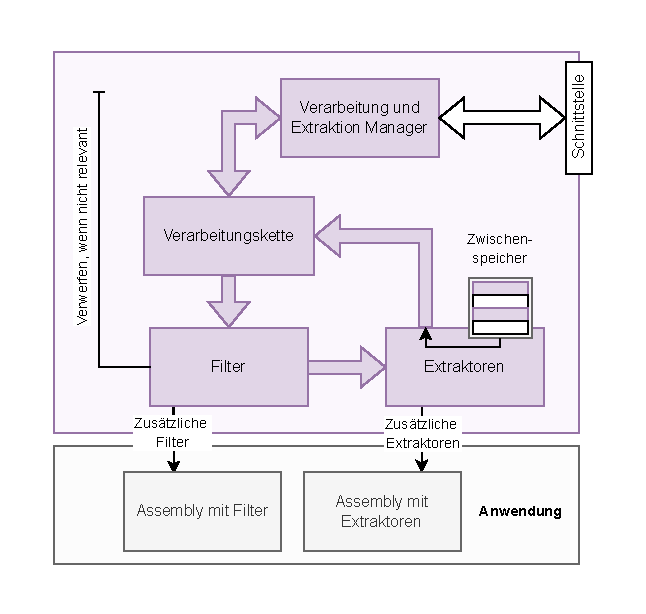
\includegraphics[width=0.6\textwidth]{5_Data_Processing_Structure.pdf}
\caption{Struktur Datenverarbeitungskomponente.}
\label{fig:structure_data_processing}
\end{figure}

\subsubsection{Manager für Verarbeitung und Extraktion}
Der Manager übernimmt, wie bereits bei den anderen Managern erwähnt, die Kommunikation mit dem übergeordneten Hauptmanager. Zusätzlich ermittelt er die Filter und Extraktoren und erzeugt die Verarbeitungskette. Er nimmt Daten asynchron entgegen und leitet diese an die Verarbeitungskette weiter. Ebenso erhält die Filterkette Extraktionsaufträge und leitet diese an die Verarbeitungskette weiter. Werden die Daten vom Hauptmanager angefordert, übergibt der Manager die extrahierten Daten aus der Verarbeitungskette. Die Hauptaufgabe des Managers liegt somit in der Datenvermittlung und der Steuerung der Verarbeitungskette, wie in Abbildung \ref{fig:structure_data_processing} veranschaulicht.

\subsubsection{Verarbeitungskette}
Die Verarbeitungskette umfasst die Filter und Extraktoren und steuert deren Initialisierung sowie Ausführung. Die Filterkette entscheidet dabei, welche Filter in welcher Reihenfolge ausgeführt werden. Die Initialisierung erfolgt primär anhand der Extraktionsaufträge, die jeder Extraktor berücksichtigen muss, um die exakt konfigurierte Datenmenge zu erhalten. Die Verarbeitungskette ist austauschbar, z.B. wenn die Strategie für die Ausführungsreihenfolge geändert werden soll.

\subsubsection{Filter}
Filter folgen einem bestimmten Schema und entscheiden, ob Daten weiterverarbeitet werden. Dies ist beispielsweise sinnvoll, wenn bestimmte Aktionen mehrfach hintereinander auftreten, aber die gleiche Bedeutung haben. Mit einem Filter können nachfolgende Aktionen für eine bestimmte Zeitspanne blockiert werden. Die eingehenden Daten, z.B. Aktionen oder sonstige Informationen, werden bei einem negativen Prüfung verworfen und an die Speicherverwaltung übergeben (siehe Abbildung \ref{fig:structure_data_processing}).

\subsubsection{Extraktoren}
Extraktoren verarbeiten Daten (Aktionen und sonstige Informationen) basierend auf den Extraktionsaufträgen. Dabei werden die Daten, die nach dem Push-Prinzip übertragen werden, genau auf die Konfiguration zugeschnitten, sodass nur relevante Daten im Ergebnis verbleiben. Die extrahierten Daten werden, wie in Unterabschnitt \ref{subsec:extraction_data_and_converting} beschrieben, weiter aggregiert und in bestimmten Objekten in vorgegebener Form abgelegt.

Um eine schnelle Aggregation und Datenübertragung bei Abruf zu gewährleisten, werden die Daten pro Extraktor gespeichert, kontinuierlich bearbeitet und im Arbeitsspeicher gehalten (siehe Abbildung \ref{fig:structure_data_processing}). Die Speicherung erfolgt im Hauptspeicher und wird nach Programmende oder durch den Garbage Collector freigegeben. Da die Daten nicht zu den primären Anwendungskomponenten gehören, können so Fehler durch externe Speicherung vermieden werden und ein Verlust der Daten hat keine Bedeutung.

\subsection{Extrahierte Daten und Weiterverarbeitung}
\label{subsec:extraction_data_and_converting}
Im Unterabschnitt \ref{subsec:communication_between_coponents} wurde beschrieben, dass die Extraktionsdaten als Kommunikationsobjekte fungieren. Genau diese Objekte werden in diesem Teil der Anwendung von den Extraktoren erzeugt. 

\subsubsection{Inhalte der Datenobjekte}
Betrachtet man die vollständige Konfiguration, so ergeben sich Objekte mit folgendem Inhalt:

\begin{itemize}
    \item \textbf{Workflow-Daten:} Enthalten den Ablauf eines Workflows als String, abgeleitet aus den Metainformationen des Extraktionsauftrags, sowie die Anzahl der Abläufe eines solchen Workflows.
    
    \item \textbf{Automatische Workflow-Daten:} Beinhalten die Aktionen innerhalb einer Ansicht, die in einem bestimmten Zeitraum in einer definierten Reihenfolge auftreten. Diese Daten dienen der weiteren Auswertung.
    
    \item \textbf{Nutzungsdaten:} Diese sind weiter unterteilt und enthalten folgende Informationen:
    \begin{itemize}
        \item \textbf{Funktionsnutzung:} Beschreibt, wie oft eine bestimmte Funktionalität aufgerufen wurde und um welche Funktion es sich handelt.
        \item \textbf{Tastaturnutzung:} Beschreibt, wie Shortcuts innerhalb einer Ansicht verwendet wurden.
        \item \textbf{Steuerelementnutzung:} Beschreibt, welche Ereignisse eines Steuerelements wie häufig auftreten.
        \item \textbf{Benutzerdefinierte Aktionen:} Beschreibt eine benutzerdefinierte Aktion sowie deren Häufigkeit des Auftretens.
    \end{itemize}
    
    \item \textbf{Metriken:} Sind numerische Werte, die weiter in folgende Kategorien unterteilt werden:
    \begin{itemize}
        \item \textbf{Ladezeiten:} Stellen aggregierte Daten zu den Ladezeiten einer Ansicht dar.
        \item \textbf{Ansichtsnutzung:} Gibt an, wie oft eine bestimmte Ansicht verwendet wurde.
    \end{itemize}
    
    \item \textbf{Kontextinformationen:} Daten, die aus einer Ansicht oder einem \textit{PresentationModel} ausgelesen werden.
\end{itemize}

\subsubsection{Weiterverarbeitung der Datenobjekte}
Um Flexibilität zu gewährleisten, können die Daten vor der Übergabe in ein eigenes Format konvertiert werden. Dadurch ist es beispielsweise möglich, die Daten anschließend für Systeme wie Google Analytics (siehe Unterabschnitt \ref{subsec:google_analytics}) weiterzuverarbeiten. 

Die gewünschte Konvertierung muss in der Systemkonfiguration (siehe Abschnitt \ref{sec:integration_concept}) angegeben werden. Für das JSON-Format existiert bereits eine Implementierung, die vom Framework bereitgestellt wird.


\section{Systemkonfiguration}
\label{sec:integration_concept}



\chapter{Implementierung}
\label{cha:implementierung}

\section{Konfiguration}
\label{sec:configuration_impl}

\section{Daten- und Aktionsermittlung}
\label{sec:data_collection_impl}

\section{Filterung und Extraktion}
\label{sec:data_extraction_impl}

\section{Integration WPF}
\label{sec:integration_wpf_impl}

\section{Integration Windows Forms}
\label{sec:integration_winforms_impl}
\chapter{Anwendung und Auswertung}
\label{cha:auswertung}

\section{Ermittlung von Verhaltensdaten}
\label{sec:testing}

\section{Auswertung und Schlussfolgerung}
\label{sec:results}

\chapter{Diskussion und Ausblick}
\label{cha:diskussion}

%%%-----------------------------------------------------------------------------
\appendix                                                               % Anhang 
%%%-----------------------------------------------------------------------------

\include{anhang.tex}

%%%-----------------------------------------------------------------------------
\backmatter                          % Schlussteil (Quellenverzeichnis und dgl.)
%%%-----------------------------------------------------------------------------

\MakeBibliography % Quellenverzeichnis

% \listoffigures
% \addcontentsline{toc}{chapter}{Abbildungsverzeichnis}

%%%-----------------------------------------------------------------------------
% Messbox zur Druckkontrolle
%%%-----------------------------------------------------------------------------

\include{back/messbox}

%%%-----------------------------------------------------------------------------
\end{document}
%%%-----------------------------------------------------------------------------
